\chapter{Coffee Time Analysis}

\todo{Basic app overview, specification}

\section{Application specification}

\todo{App domain}

\section{Existing alternatives}
The analysis of existing alternatives was made to research already created applications with similar features. Existing applications were searched through Android's official store. Applications with these functionalities were chosen for the review.

\begin{itemize}
    \item Nearby place search
    \item Application's theme should be cafes or similar
\end{itemize}

For comparison five, the most inspiring and distinguish applications were chosen. The following lines briefly describe one of each, their target audience, the advantages and drawbacks. 

\subsection{Gastromapa Lukáše Hejlíka}
\todo{LINK}
Published in the first quarter of 2019 as a new application for exploring restaurants in the Czech Republic.  The application's speciality is that restaurants' reviews are not done by users but by gastronomy specialist \textit{Lukáš~Hejlík}.

As soon as the application launches, it displays nearby restaurants. Each establishment is shown as a card with important information such as an address, distance and type of restaurant. The main card's domain is a large photo which should catch the user's eye to take a look. 

After the card is clicked, the user is presented with the restaurant's detail, where more information such as opening hours, map location and comprehensive review by~\textit{L.~Hejlík} can be found. From this detail navigation to the chosen restaurant can be launched. The target audience is anyone who seeks to visit unknown places and possess the opportunity to taste great food.

\begin{figure}[h]
    \centering
    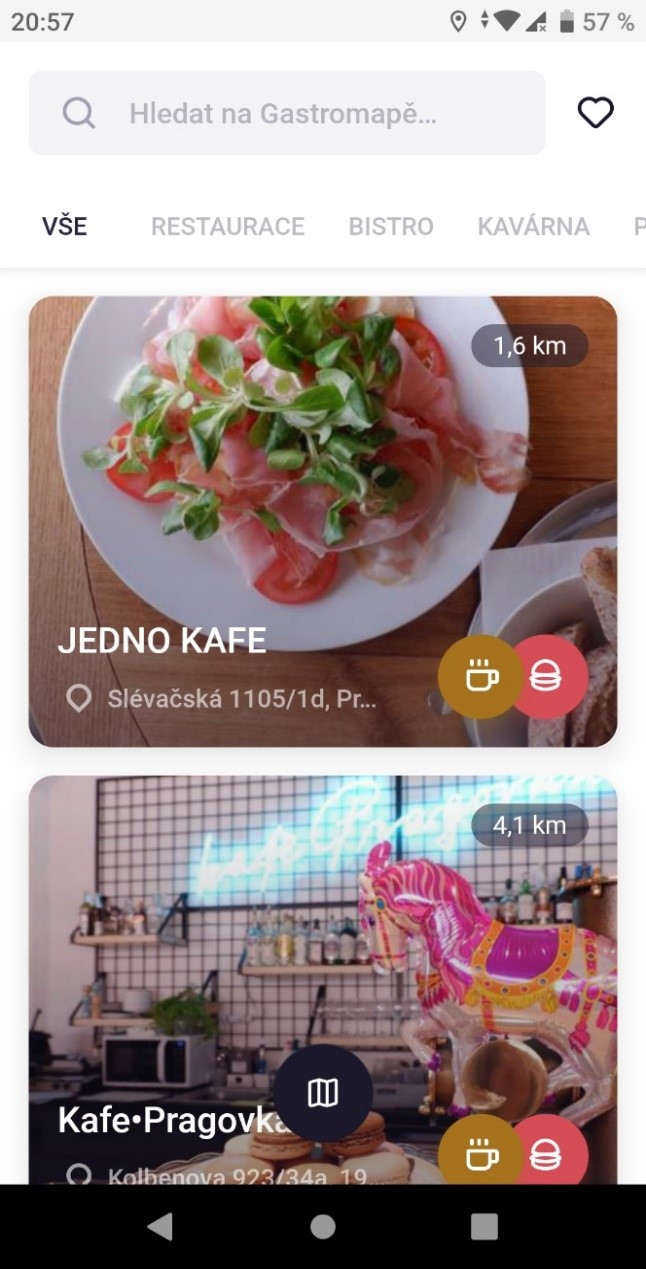
\includegraphics[width=0.33\linewidth]{img/analysis/gastromapa_hejlik.jpg}
    \caption{Gastromapa \textit{L. Hejlíka} \todo{Include app's images?}}
    \label{fig:Gastromapa L. Hejlika}
\end{figure}

\subsubsection{The advantages}
\begin{itemize}
    \item Design is fresh, clean and users can immediately see relevant content.
    \item Thanks to clean design application is easy to use and understand.
    \item The whole application behaves smoothly without any noticeable freezing.
\end{itemize}

\subsubsection{The drawbacks}
\begin{itemize}
    \item The navigation button has a blackish colour that after scrolling disappears. If the restaurant has a darker photo, the button is hard to notice. 
    \item When coming back to the main screen, loading of the list is started again, and the previous search is lost.
    \item Detail screen on entry is fully covered with restaurant photo. From a design point of view, it is a nice touch, but users must scroll to see any information. 
\end{itemize}

\subsection{Pivní deník}
\todo{LINK} Application \textit{Pivní deník} is used to search nearby restaurants in the Czech Republic focused on beers. The content is created by the community, including served beers and their prices.  Application offers searching nearby restaurants filtering them by served type of beer. Each user has a history of visited places, can mark restaurant as favourite and propagate their favourite brands.

\subsubsection{The advantages}
\begin{itemize}
    \item Brasseries are displayed as a list or on the map view.
    \item The served brands are displayed directly within the list, so it is not needed to visit details.
    \item The registration is optional for searching. If users want to contribute, they must have an account.
\end{itemize}

\subsubsection{The drawbacks}
\begin{itemize}
    \item Registration can be done through Facebook or e-mail. With e-mail registration, the user is redirected to the web page where registration is finished.
    \item As was said, content is created by the community. During the research, it was clear that many information is outdated or misleading. 
    \item Overall application design looks outdated and does not meet current, modern,  trends.
    \item On the primary screen user's stats like the number of drunken beers and at most three nearest restaurants are displayed. On the larger screens, there is plenty of unused space. 
    \item Each restaurant displays only one brand of drafted beer. Nowadays, many restaurants offer more than one brand. 
    \item Side menu can be opened only with the hamburger icon but not with slide to right gesture.
\end{itemize}

\subsection{Restu}
\todo{LINK} Restu is another gastronomy guide focused on restaurants in the Czech Republic.  Through the application, reservations can also be made.
Target audience is everyone who searches for new places where to eat and make a reservation. 
Application has many original functionalities. For example ``discover'' section which shows attractive offers, the best cafe in the city and similar. Another is the ``check-in'' button which gave credits to users if they eat at the given restaurant.

\subsubsection{The advantages}
\begin{itemize}
    \item Clean and well-structured layout.
    \item Opt-in registration.
\end{itemize}

\subsubsection{The drawbacks}
\begin{itemize}
    \item When business card selected small bottom info windows is displayed but cannot be hidden again.
    \item To review restaurant user has to be signed in and the restaurant must be open. If closed, the review cannot be added.
\end{itemize}

\subsection{Zomato}
\todo{LINK} Zomato is primarily web-based restaurant browser in the world. It has its own database of establishments. Content is edited by users.  
On the primary screen are displayed ``week hits'', top restaurants or for example ``happy hours''. Restaurants are divided into categories such as ``Nightlife'' or ``Daily menu'' which helps for navigation within the application.
Target audience is anyone who wants to try new restaurants or looking for action offers. 

\subsubsection{The advantages}
\begin{itemize}
    \item Well solved filtering. Filter setting is intuitive, displays most used filters. 
    \item Advanced options for filtering with tags such as ``dog friendly'' or ``WiFi free''.
    \item Friendships with other users. If another user added review notification is received.
\end{itemize}

\subsubsection{The drawbacks}
\begin{itemize}
    \item The primary screen is cluttered with many information at one place.
    \item Nearby restaurants list is hidden below ``favourites restaurants'' and ``month collections''.
    \item Full-text search in some circumstances behaves unexpectedly. For example, to search for restaurants which offer ``asian food'' user has to type exactly ``asian'' but not ``asia''.
    \item Readability of some text is worsened by light background and greyish text colour. In some scenarios, such as reading outside, is hard to read.
\end{itemize}

\subsection{Google maps}
\todo{LINK}

\section{Lofi / Hifi prototype}
\todo{Use results from MI-NUR. User prototype testing and results}

\todo{Use cases, diagrams, architecture}

\subsection{Nielsen heuristic}
\todo{Nielsen heuristic evaluation}

\section{Technical analysis}

\subsection{Google Places API}
\todo{Google places API and how it is used.}

\section{Serverless approach \todo{Maybe move it to another chapter before analysis?}}

\todo{Firebase. Cloud functions. Firestore - NoSQL document based database. Pricing}
\blind[2]



